\documentclass[12pt]{beamer}
\usepackage[utf8]{inputenc} % style d'écriture
\usepackage[T1]{fontenc}      % package
\usepackage[french]{babel}  % package pour langue française
\usepackage{graphicx}
\usepackage{subcaption}
\usepackage{url}
\usepackage{color}
\usepackage{geometry}
\usepackage{amssymb}
\usepackage{multirow, makecell}
\usepackage{listings}

% William PENSEC, étudiant en Master 2 LSE 2020/2021

\usetheme[secheader]{Madrid}
\beamertemplatenavigationsymbolsempty
\setbeamertemplate{frametitle continuation}{}

\lstset{
  aboveskip=5mm,
  belowskip=-2mm,
  basicstyle=\footnotesize,
  breakatwhitespace=false,
  breaklines=true,
  captionpos=b,
  commentstyle=\color{red},
  deletekeywords={...},
  escapeinside={\%*}{*)},
  extendedchars=true,
  framexleftmargin=16pt,
  framextopmargin=3pt,
  framexbottommargin=6pt,
  frame=tb,
  keepspaces=true,
  keywordstyle=\color{blue},
  language=C++,
  literate=
  {²}{{\textsuperscript{2}}}1
  {⁴}{{\textsuperscript{4}}}1
  {⁶}{{\textsuperscript{6}}}1
  {⁸}{{\textsuperscript{8}}}1
  {€}{{\euro{}}}1
  {é}{{\'e}}1
  {è}{{\`{e}}}1
  {ê}{{\^{e}}}1
  {ë}{{\"{e}}}1
  {É}{{\'{E}}}1
  {Ê}{{\^{E}}}1
  {û}{{\^{u}}}1
  {ù}{{\`{u}}}1
  {â}{{\^{a}}}1
  {à}{{\`{a}}}1
  {á}{{\'{a}}}1
  {ã}{{\~{a}}}1
  {Á}{{\'{A}}}1
  {Â}{{\^{A}}}1
  {Ã}{{\~{A}}}1
  {ç}{{\c{c}}}1
  {Ç}{{\c{C}}}1
  {õ}{{\~{o}}}1
  {ó}{{\'{o}}}1
  {ô}{{\^{o}}}1
  {Õ}{{\~{O}}}1
  {Ó}{{\'{O}}}1
  {Ô}{{\^{O}}}1
  {î}{{\^{i}}}1
  {Î}{{\^{I}}}1
  {í}{{\'{i}}}1
  {Í}{{\~{Í}}}1,
  morekeywords={*,...},
  numbers=left,
  numbersep=10pt,
  numberstyle=\tiny\color{black},
  rulecolor=\color{black},
  showspaces=false,
  showstringspaces=false,
  showtabs=false,
  stepnumber=1,
  stringstyle=\color{gray},
  tabsize=4,
  title=\lstname,
}

\title[Compte rendu de stage n\textsuperscript{o}15]{Coopération de drones dans un système hétérogène}
\subtitle{Compte rendu de stage n\textsuperscript{o}15}
\author{William \textsc{Pensec}}
%\author{William \textsc{Pensec}}
%\author{William \textsc{Pensec}}
\institute[Lab-STICC]{Lab-Sticc}
\date{\today}

%\AtBeginSection[]
%{
%\begin{frame}<beamer>{Sommaire}
%\tableofcontents[currentsection,currentsubsection, 
%    hideothersubsections, 
%    sectionstyle=show/shaded,
%]
%\end{frame}
%}

\begin{document}
	% ---------------------------------------------------------------- %
	\begin{frame}
		\begin{titlepage}
			\begin{figure}[H]
				\centering
				
\includegraphics[scale=.15]{labsticc.png}
				\hspace{3cm}
				
\includegraphics[scale=.3]{ubo.png}
			\end{figure}
		\end{titlepage}
	\end{frame}
	
	% ---------------------------------------------------------------- %
	\section*{Sommaire}
	\begin{frame}
		\frametitle{Sommaire}
		\begin{center}
			\tableofcontents
		\end{center}
	\end{frame}
	%
	% ---------------------------------------------------------------- %
	\section{LabelImg}
	\begin{frame}[allowframebreaks]
	    \frametitle{LabelImg}
	     \begin{block}{Utilisation du logiciel LabelImg}
	        \begin{itemize}
	            \setbeamertemplate{itemize item}[triangle]
	            \item Logiciel libre
	            \item Écrit en python
	            \item Sert pour Yolo \& PascalVOC
	            \item \url{https://github.com/tzutalin/labelImg}
	            \item Ecrit un fichier texte sous forme : classe centreX centreY largeur hauteur
	        \end{itemize}
	    \end{block}
    \end{frame}
	%
	% ---------------------------------------------------------------- %
	\begin{frame}[allowframebreaks]
	    \begin{figure}
		    \centering
		    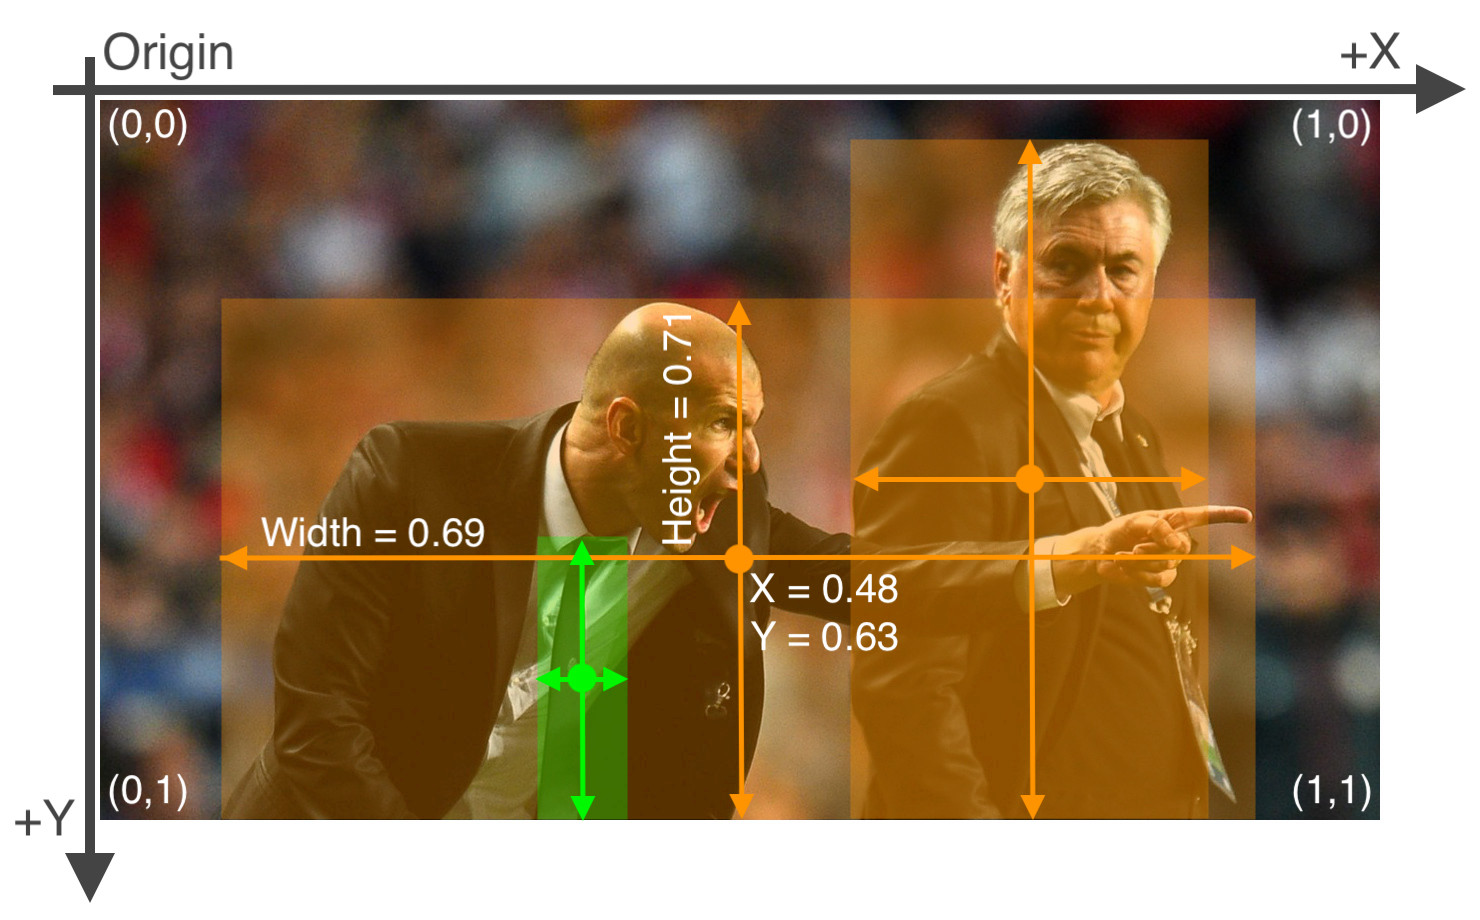
\includegraphics[width=1\linewidth]{image/exempleImgYolo.png}
	    \end{figure}
	    
	    \begin{figure}
		    \centering
		    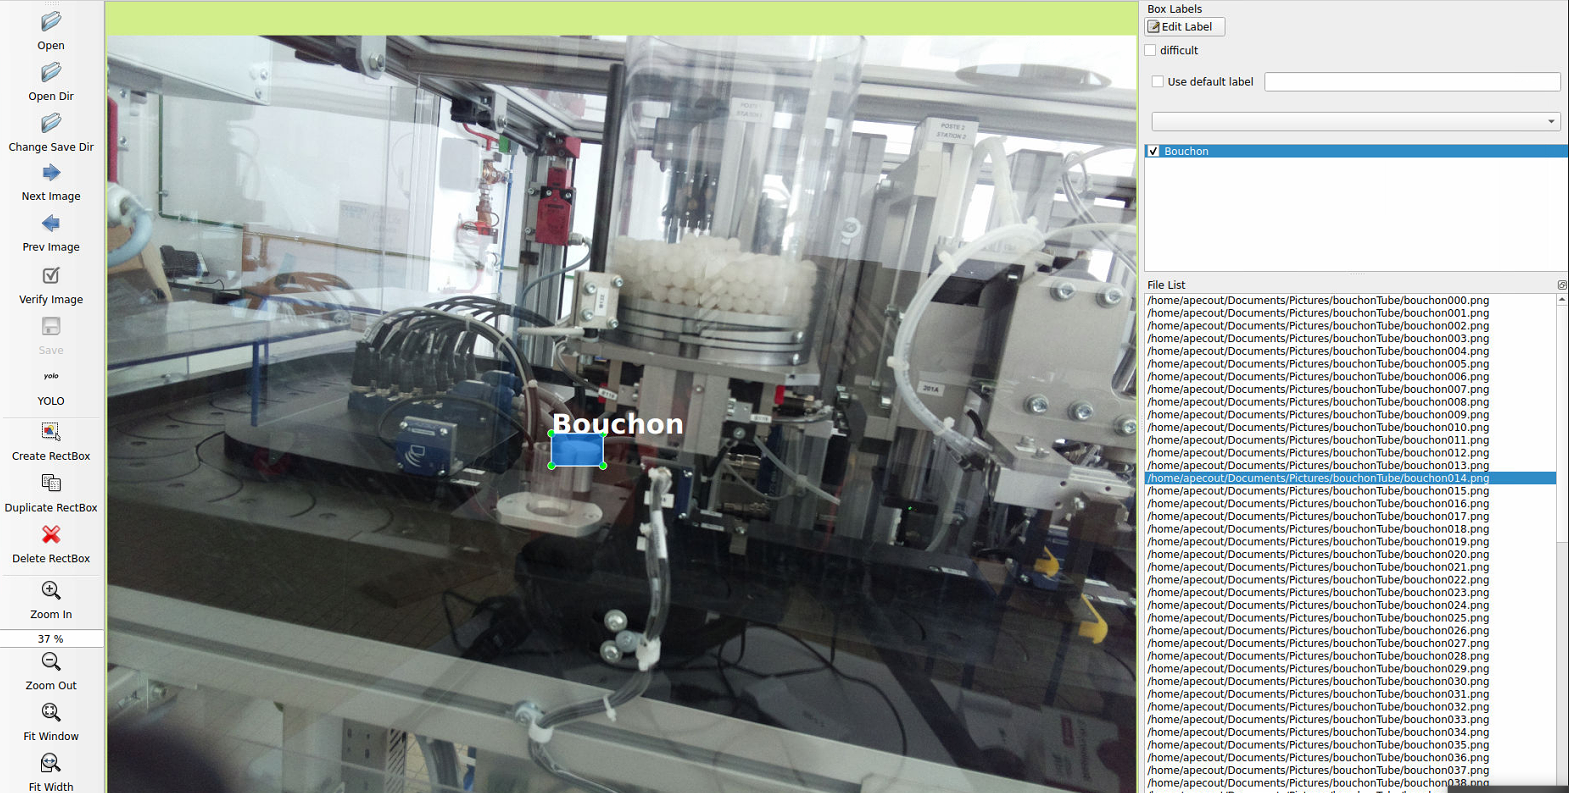
\includegraphics[width=1\linewidth]{image/labelImg.png}
	    \end{figure}
	    
	    \begin{figure}
		    \centering
		    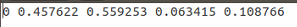
\includegraphics[width=1\linewidth]{image/labelTxt.png}
	    \end{figure}
	\end{frame}
	%
	% ---------------------------------------------------------------- %
	\section{Yolo}
	\subsection{Présentation}
	\begin{frame}[allowframebreaks]
	\frametitle{Yolo - Présentation}
	    \begin{block}{Utilisation de YoloV5}
	        \begin{enumerate}
	            \setbeamertemplate{itemize item}[triangle]
	            %\item \url{https://github.com/ultralytics/yolov5}
	            \item Création d'un fichier YAML afin d'indiquer le nombre de classes, les classes, le chemin d'accès aux images pour entrainer, valider et tester le réseau
	            \item Séparation entre deux dossiers pour stocker labels et images:
	                \begin{itemize}
	                    \item Dossier \textit{labels/}
	                    \item Dossier \textit{images/}
	                \end{itemize}
	            \item Sélection du modèle Yolov5 (voir figure 1)
	            \item Entrainement du modèle avec la commande : \textit{python train.py --img 640 --batch 2 --epochs 30 --data plateforme.yaml --weights yolov5s.pt --nosave --cache}
	            \item Visualiser les résultats
	        \end{enumerate}
	    \end{block}
    \end{frame}
	%
	% ---------------------------------------------------------------- %
    \begin{frame}[allowframebreaks]    
	    \begin{figure}
		    \centering
		    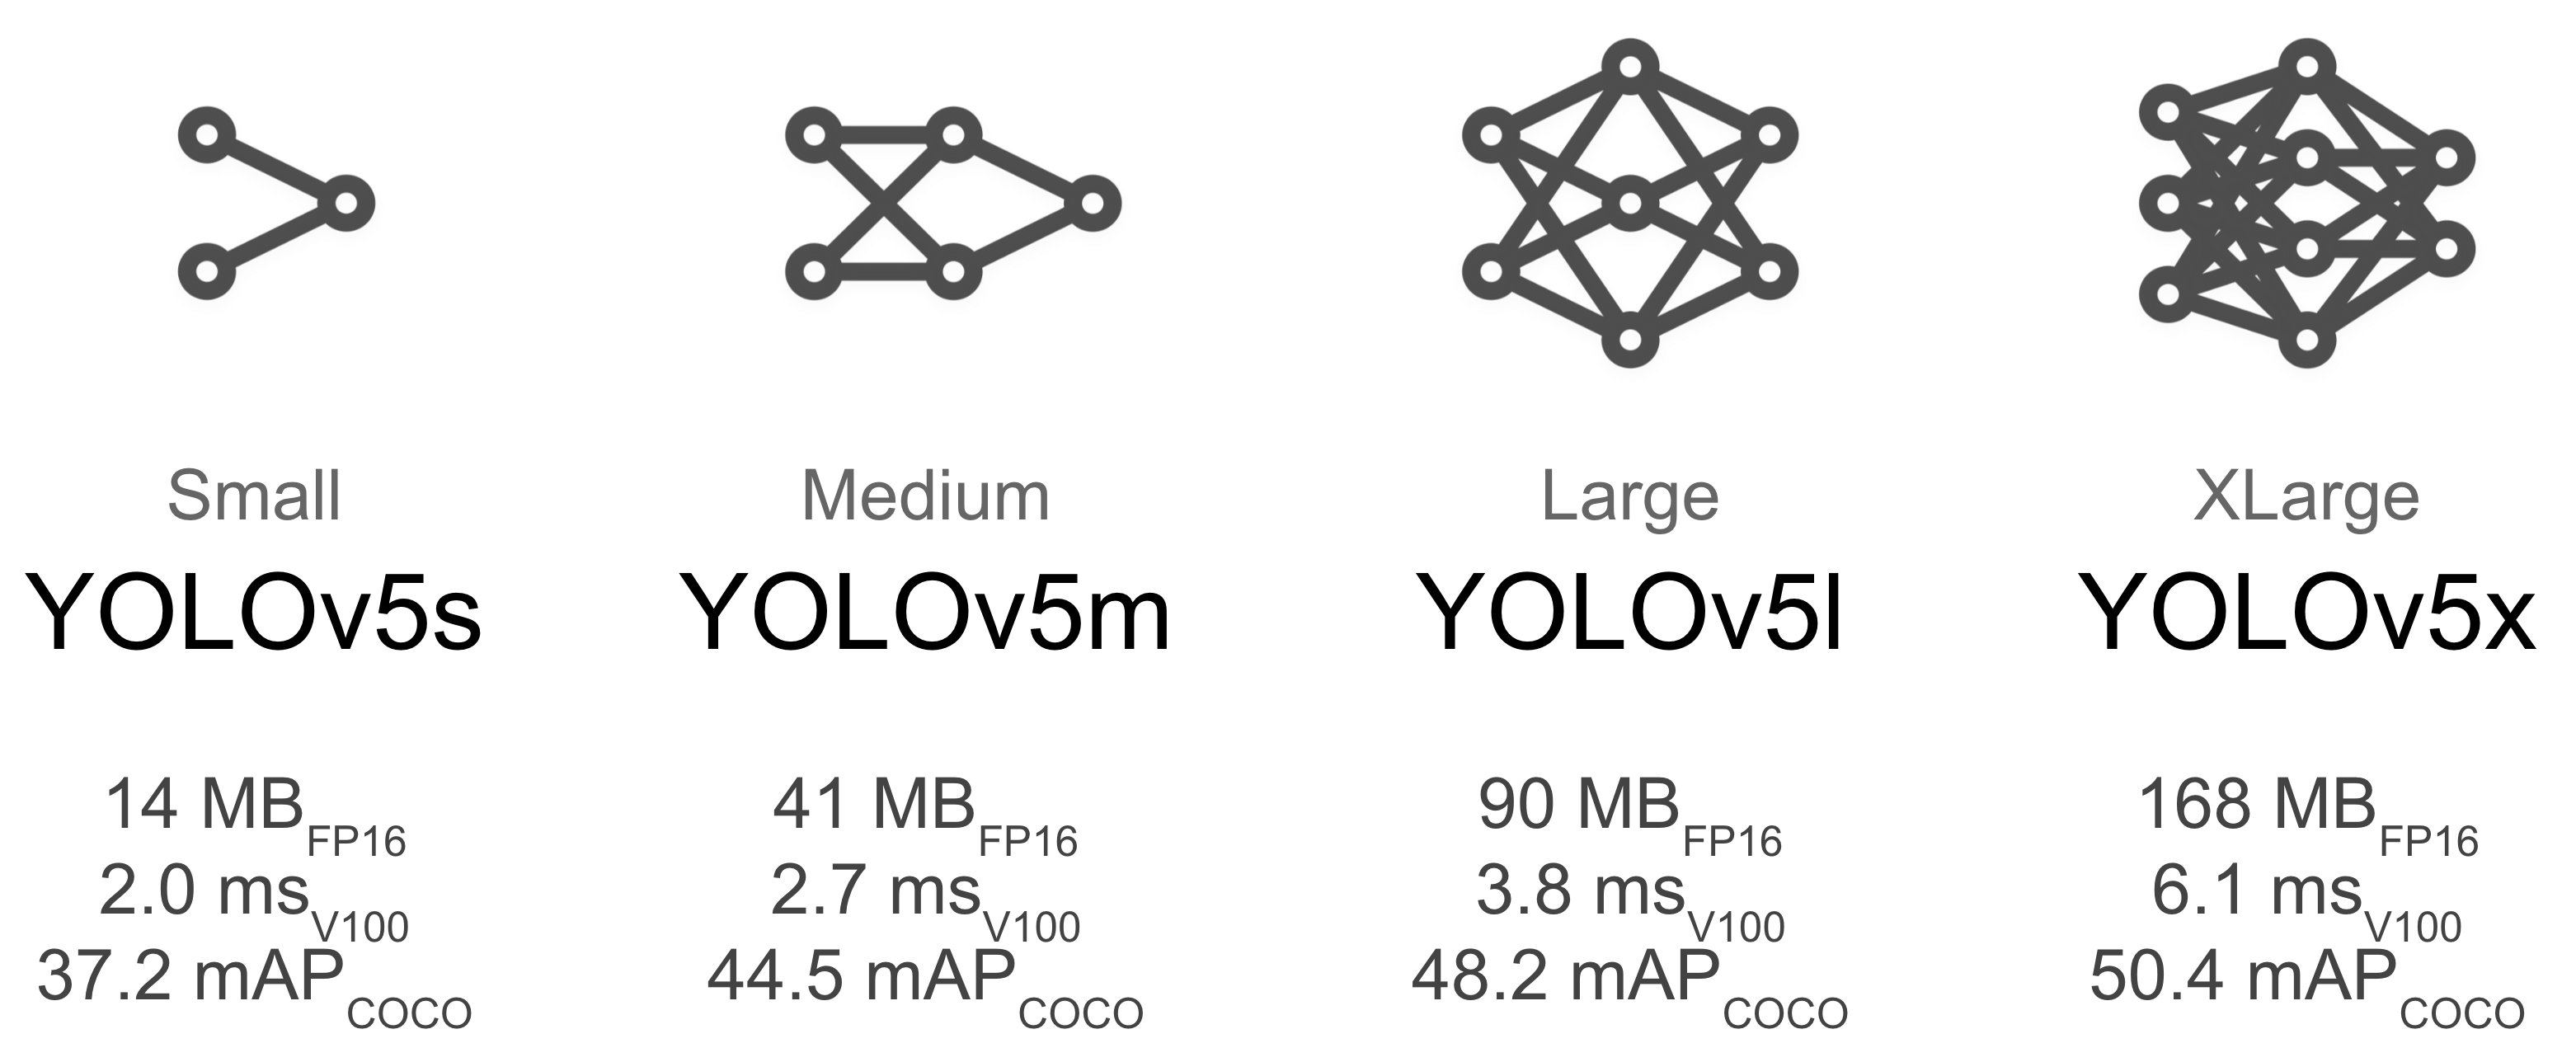
\includegraphics[width=0.8\textwidth]{image/yolov5.png}
		    \caption*{\label{fig:modeleYolov5}Différents modèles existants}
	    \end{figure}
	    
	    \begin{figure}
		    \centering
		    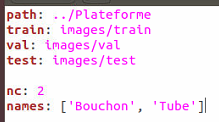
\includegraphics[width=0.65\textwidth]{image/yaml.png}
	    \end{figure}
	\end{frame}
	%
	% ---------------------------------------------------------------- %
	\subsection{Résultats}
    \begin{frame}[allowframebreaks]
        \begin{block}{Utilisation de YoloV5 - Temps d'exécution sur Serveur (8 coeurs, 50Go de RAM)}
	        \begin{itemize}
	            \setbeamertemplate{itemize item}[triangle]
	            \item 30 epochs, yolov5s.pt -> 20 minutes 
	            \item 50 epochs, yolov5s.pt -> 35 minutes
	            \item 30 epochs, yolov5l.pt -> 1h32
	            \item 60 epochs, yolov5x.pt -> environ 13h
	        \end{itemize}
	    \end{block}
    
    
	    \begin{figure}
		    \centering
		    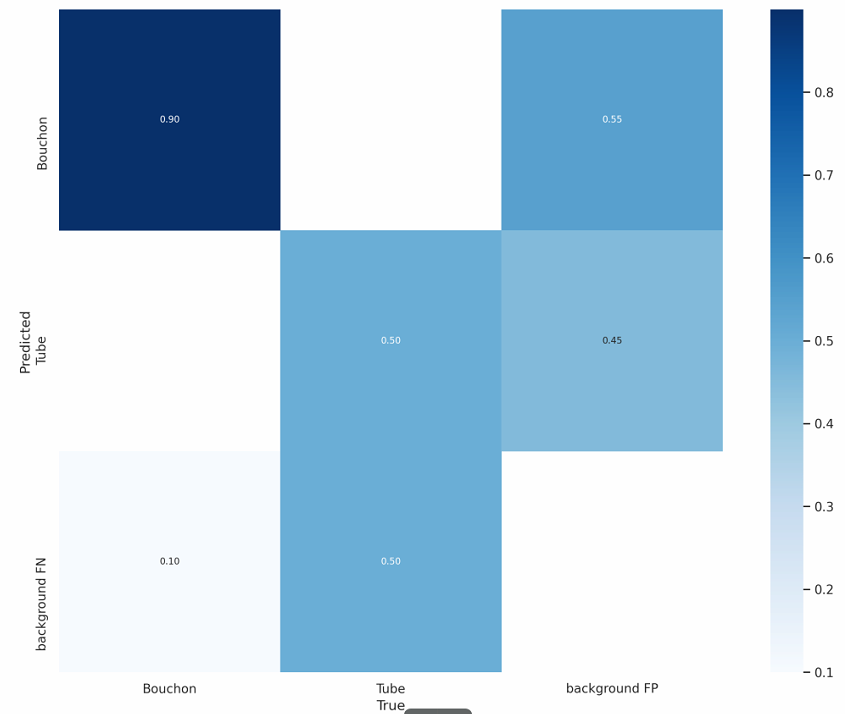
\includegraphics[width=0.75\textwidth]{image/confusionsMatrix.png}
		    \caption*{30 epochs, yolov5s}
	    \end{figure}
	    
	    \begin{figure}
		    \centering
		    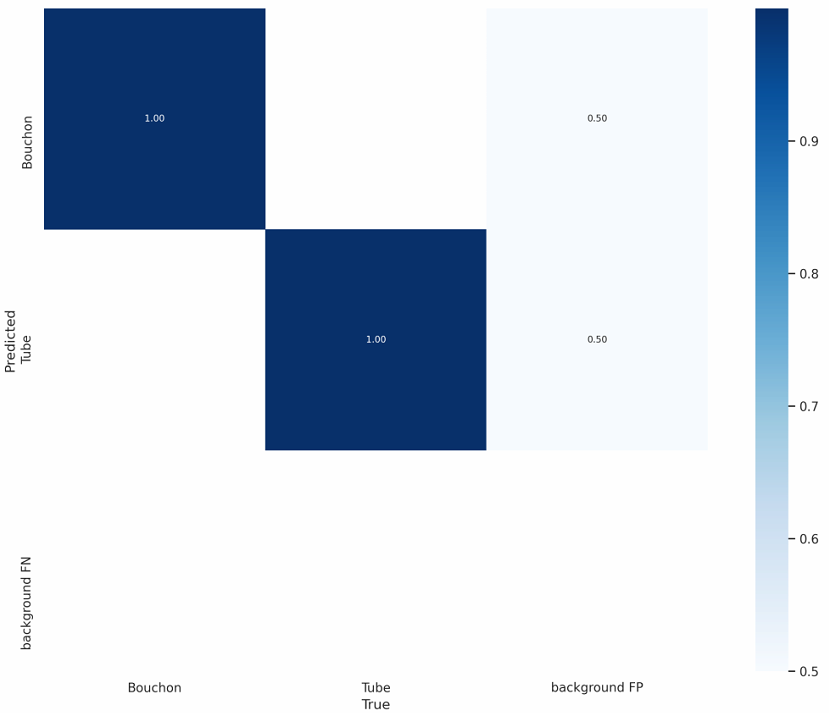
\includegraphics[width=0.75\textwidth]{image/confusionMatrixBest.png}
		    \caption*{60 epochs, yolov5x}
	    \end{figure}
	    
	    
	    \begin{figure}
		    \centering
		    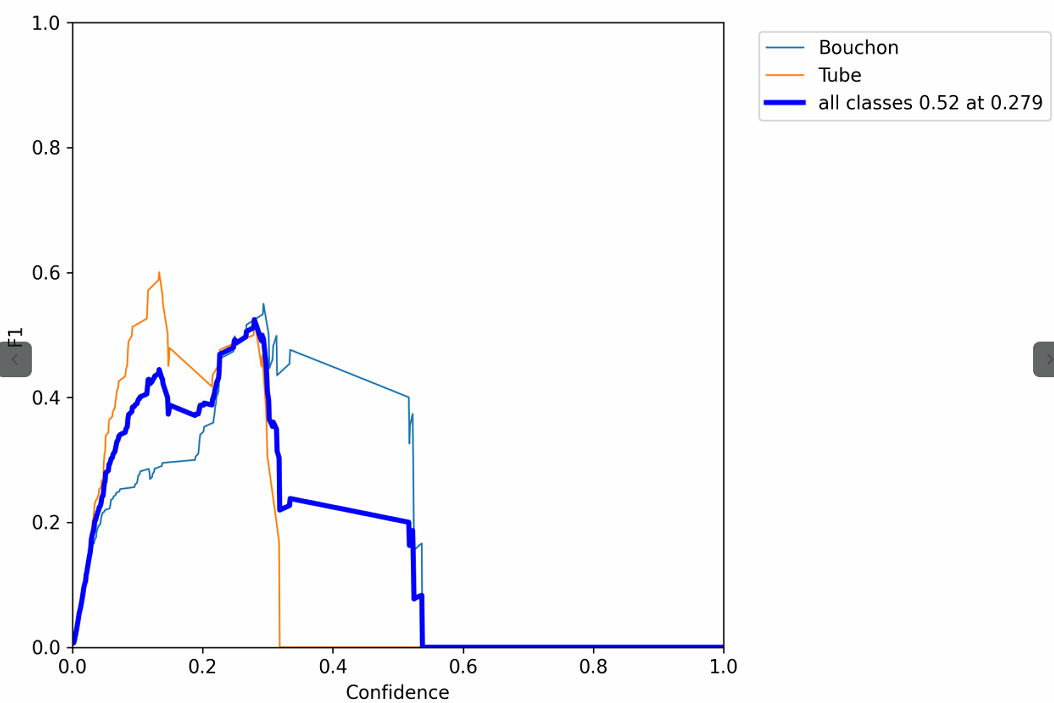
\includegraphics[width=0.9\textwidth]{image/curve13.png}
		    \caption*{30 epochs, yolov5s}
	    \end{figure}
	    
	    \begin{figure}
		    \centering
		    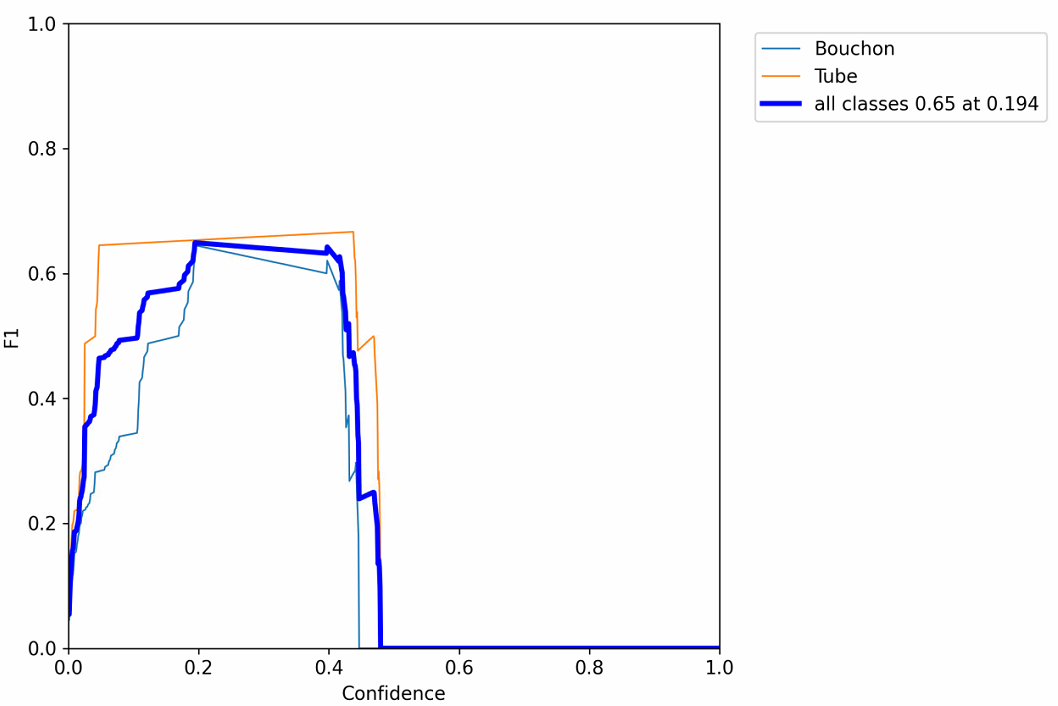
\includegraphics[width=0.9\textwidth]{image/curve10.png}
		    \caption*{60 epochs, yolov5x}
	    \end{figure}
	\end{frame}
	%
	% ---------------------------------------------------------------- %
	\begin{frame}[allowframebreaks]
	    \begin{alertblock}{A tester}
	        \begin{itemize}
	            \setbeamertemplate{itemize item}[triangle]
	            \item Batch plus grands (95 photos => 19 batchs * 5 images ...)
	            \item Epochs à faire varier
	            \item Peut être + d'images ? Et différentes images
	        \end{itemize}
	    \end{alertblock}
	\end{frame}
	%
	% ---------------------------------------------------------------- %
\end{document}